\begin{figure}[htbp]
  \centering
  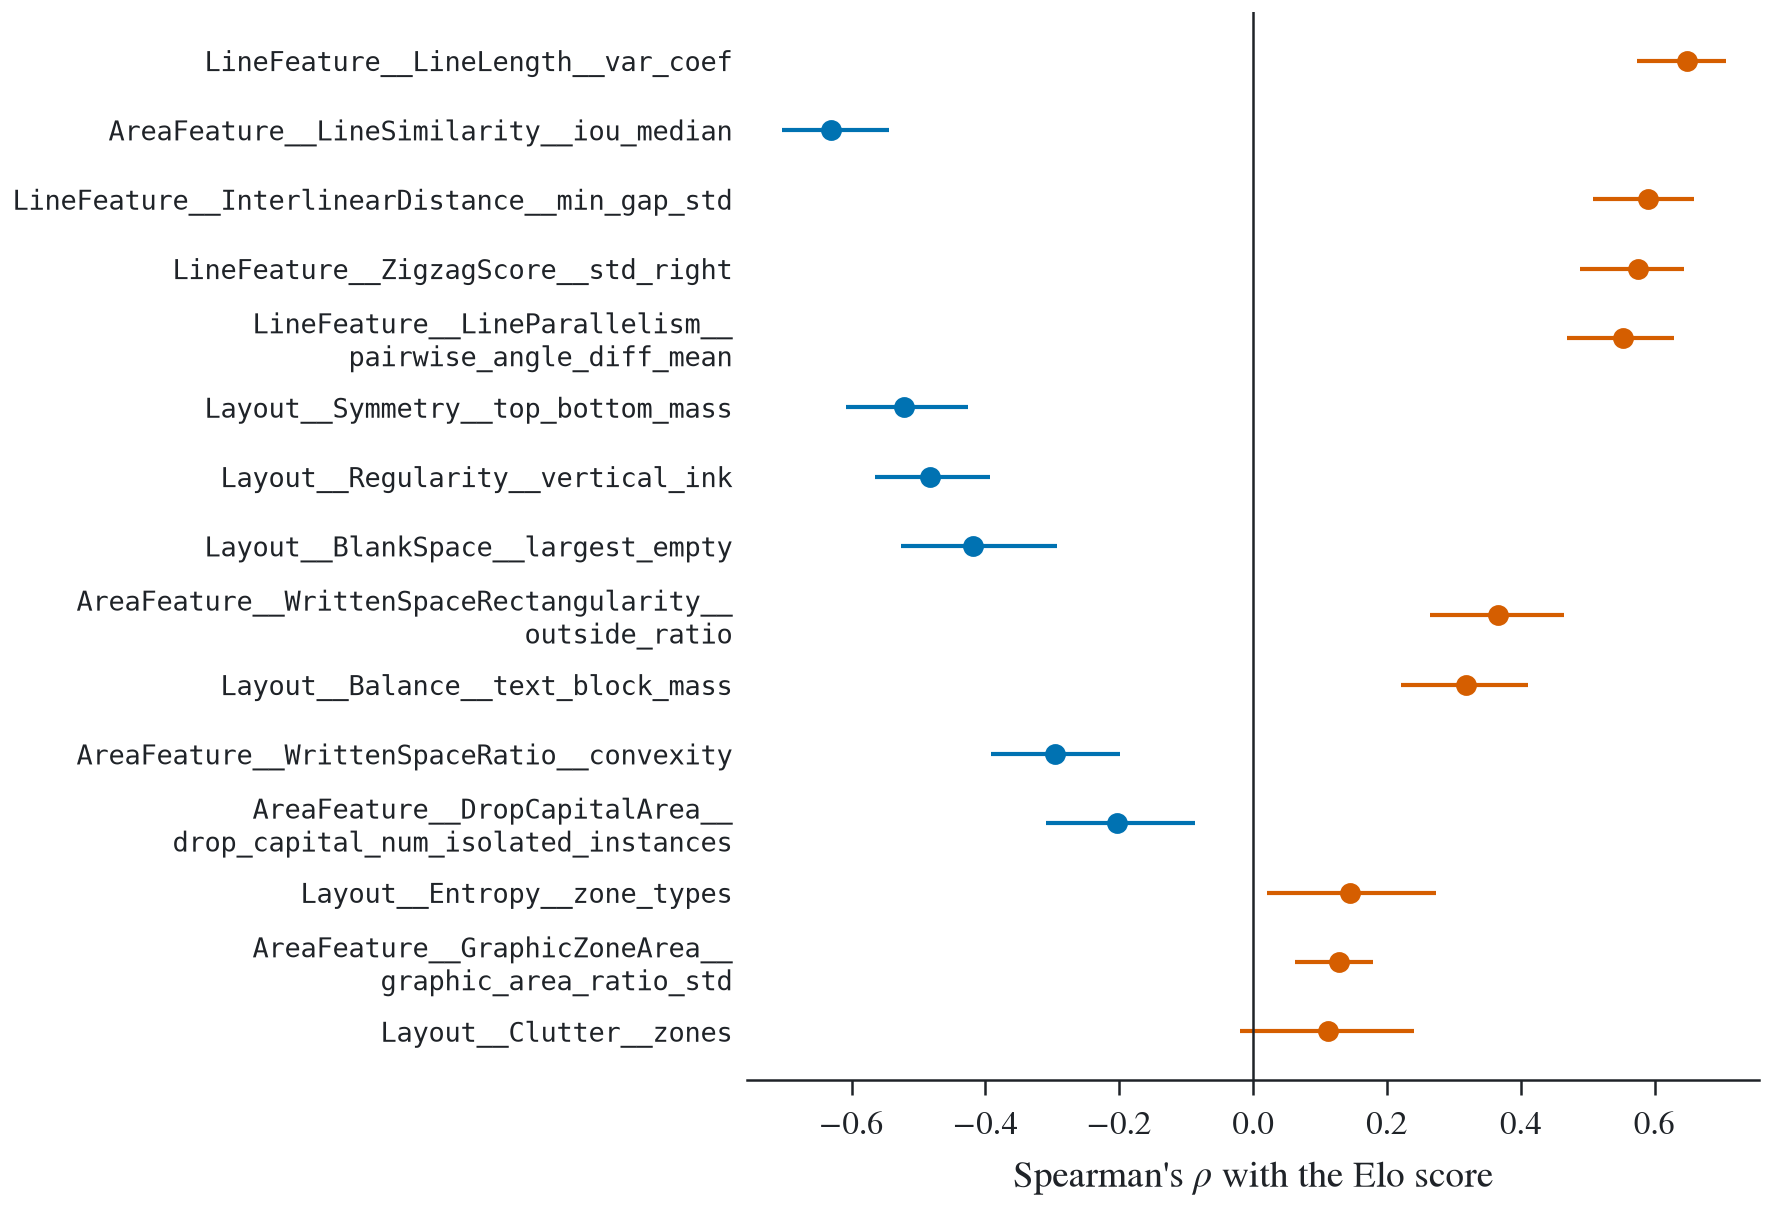
\includegraphics[width=15.00cm]{figures/geometry_feature_correlations.png}
  \caption{Spearman's correlation ($\rho$) between each feature's best flavour (the one whose correlation is strongest) and the pages' Elo scores, over the 397 pages, with 95\% intervals from 1,000 resamples of the manuscripts; blue where negative, vermillion where positive. From top to bottom: \texttt{LineFeature\_\_LineLength\_\_var\_coef}, the coefficient of variation of the baselines' lengths relative to their zone's width; \texttt{AreaFeature\_\_LineSimilarity\_\_iou\_median}, the median IoU similarity of two line polygons centred on each other; \texttt{LineFeature\_\_InterlinearDistance\_\_min\_gap\_std}, the standard deviation of the shortest distance between consecutive baselines; \texttt{LineFeature\_\_ZigzagScore\_\_std\_right}, the standard deviation of the lines' right offsets from their zone's edge; \texttt{LineFeature\_\_LineParallelism\_\_pairwise\_angle\_diff\_mean}, the mean of the absolute differences between two baselines' angles; \texttt{Layout\_\_Symmetry\_\_top\_bottom\_mass}, the mirror symmetry of the written mass about the text block's horizontal axis; \texttt{Layout\_\_Regularity\_\_vertical\_ink}, the highest vertical autocorrelation peak of the ink; \texttt{Layout\_\_BlankSpace\_\_largest\_empty}, the largest empty rectangle relative to the folio; \texttt{AreaFeature\_\_WrittenSpaceRectangularity\_\_outside\_ratio}, the share of the written space outside a rectangle of its area and the folio's proportions; \texttt{Layout\_\_Balance\_\_text\_block\_mass}, the distance of the written mass's centre from the text block's centre; \texttt{AreaFeature\_\_WrittenSpaceRatio\_\_convexity}, the area of the union of the line polygons relative to its convex hull's; \texttt{AreaFeature\_\_DropCapitalArea\_\_drop\_capital\_num\_isolated\_instances}, the number of separate drop capitals; \texttt{Layout\_\_Entropy\_\_zone\_types}, the entropy of the zone types' shares of the zones' area; \texttt{AreaFeature\_\_GraphicZoneArea\_\_graphic\_area\_ratio\_std}, the standard deviation area of the graphic zones, each relative to the folio's; \texttt{Layout\_\_Clutter\_\_zones}, the number of zones on the folio.}
  \label{fig:geometry_feature_correlations}
\end{figure}
